\begin{problem}[15]
分析小球在粘性流体中下落的最终速度和粘性阻力(把结果与Stokes公式做对比).
\end{problem}
% --------------------------------------------------------------------
\begin{solution}
\begin{minipage}[c]{0.8\linewidth}
\textbf{最终速度:} 小球在粘性流体中下落的最终速度$v$, 与小球的直径$d$和密度$\rho_\mathrm{s}$, 流体的密度$\rho$和粘性系数$\mu$, 以及重力加速度$g$有关. 显然对于小球的最终速度, 小球的密度$\rho_\mathrm{s}$和流体的密度$\rho$是以差的形式出现的, 因此有
\[
v = f(\rho_\mathrm{s}-\rho, d, \mu, g)
\]
上式中各物理量的量纲分别为: $[v]=LT^{-1}$, $[\rho_\mathrm{s}-\rho]=ML^{-3}$, $[d]=L$, $\mu=ML^{-1}T^{-1}$, $[g]=LT^{-2}$. 以$\rho_\mathrm{s}-\rho$, $\mu$和$d$为基本量, 并作为本问题的单位系统, 来度量问题中的各量, 于是上式转化为
\end{minipage}
\begin{minipage}[c]{0.2\linewidth}
\begin{center}
\usetikzlibrary{calc,intersections,through,backgrounds}
\usetikzlibrary{decorations.pathreplacing,decorations.pathmorphing,arrows}
\usetikzlibrary{shadows}
\begin{tikzpicture}


\node at (0,0) {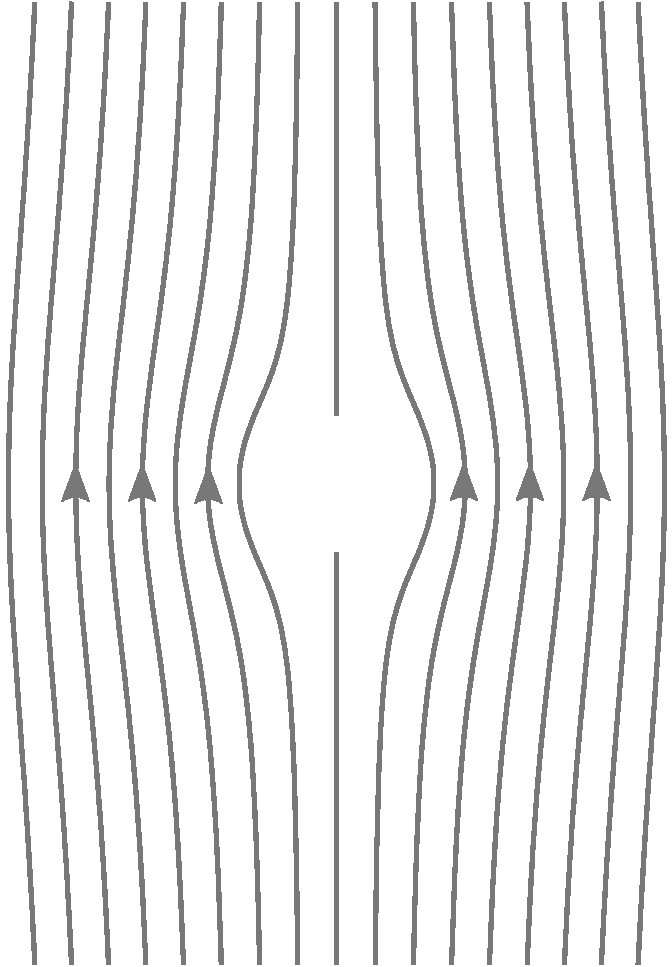
\includegraphics[width=75pt]{./figures/Stokes_sphere.pdf}};
\shadedraw [ball color= gray!30,thick] (0,0) circle (0.3);
\draw[blue,thick](0.6,0.3) -- (0.9,0.3) (0.6,-0.3) -- (0.9,-0.3);
\draw[blue,thick,<->,>=stealth](0.75,0.3) -- (0.75,-0.3) node[right, midway] {$d$};
\node[blue] at (0,0) {$\rho_\mathrm{s}$};
\draw[blue,->, >=stealth, thick](-0.75,-0.3) -- (-0.75,-1) node[below]{$g$};
\draw[blue] (-0.75,0.5) node{$\rho$, $\mu$};
\draw[blue,->, >=stealth, thick] (0,-0.3)--(0,-1) node[below] {$G$};
\draw[blue,->, >=stealth, thick] (0,0.3)--(0,1) node[above] {$F_\mathrm{b}+F_\mathrm{v}$};

\end{tikzpicture}

\end{center}
\end{minipage}\vspace{5pt}
\[
\frac{v}{\mu/[(\rho_s-\rho)d]} = f\bigg(1,1,1,\frac{g}{\mu^2/[(\rho_s-\rho)^2 d^3]}\bigg) 
\quad\Longrightarrow\quad
v = \frac{\mu}{(\rho_s-\rho)d}f\bigg(\frac{g(\rho_s-\rho)^2d^3}{\mu^2}\bigg)
\]
从\textcolor{blue}{粘性阻力}(见下文式\ref{eq:15Fv-eq-cuvd})的分析中可知, 最终小球所受粘性阻力$F=C\mu v d$为常数, 即$\mu$与$v$成反比, 因此上式可化简为
\[
v = C\cdot\frac{\mu}{(\rho_s-\rho)d} \cdot \frac{g(\rho_s-\rho)^2d^3}{\mu^2} 
= C\cdot\frac{\rho_s-\rho}{\mu} d^2 g
\]
其中$C$为常数, 对比由Stokes公式得到的结果: $v = \frac{(\rho_s-\rho)gd^2}{18\mu}$, 可知上式中$C$的值为$C = 1/18$.

\vspace{10pt}

\noindent\textbf{粘性阻力:} 小球在粘性流体中下落平衡后速度为定值$v$. 粘性阻力$F_\mathrm{v}$最终将恒定, 与小球直径$d$, 流体的密度$\rho$和粘性系数$\mu$, 及最终下落速度$v$有关:
\[
F_\mathrm{v} = f(\rho, \mu, v, d)
\]
其中$F_\mathrm{v}$的量纲为$[F_\mathrm{v}]=MLT^{-2}$. 选取$\mu$, $v$和$d$为基本量, 并作为本问题的单位系统, 来度量问题中的各量, 于是上式转化为
\begin{equation}\label{eq:15Fv-eq-cuvd}
\frac{F_\mathrm{v}}{\mu vd} = f\bigg(\frac{\rho v d}{\mu},1,1,1\bigg)
\quad\Longrightarrow\quad
F_\mathrm{v} = f(\mathrm{Re}) \mu vd
\end{equation}
该问题的雷诺数$\mathrm{Re}\ll 1$, 因此$f(\mathrm{Re})=C$为常数. 对比由Stokes公式得到的结果: $F_\mathrm{v} = 3\pi \mu vd$, 可知常数$C=3\pi$.
\vspace{10pt}

\noindent\textcolor{blue}{从另一角度, 也可求得粘性阻力}. 小球在粘性流体中下落平衡后速度为定值, 则所受重力$G$和浮力$F_b$, 粘性阻力$F_v$平衡, 即 
\begin{equation}\label{eq:15Fv-eq-G-Fb}
F_v = G - F_b = \rho_s V g - \rho V g = \frac{1}{6}\pi (\rho_s - \rho) d^3 g
\end{equation}
进一步由式(\ref{eq:15Fv-eq-cuvd})和式(\ref{eq:15Fv-eq-G-Fb})也可求得小球在粘性流体中下落的最终速度
\[
v = \frac{1}{18}\frac{\rho_s-\rho}{\mu} d^2 g, \qquad
\mu = \frac{1}{18}\frac{\rho_s-\rho}{v}d^2 g
\]
利用上右式可用来测定未知流体的粘性系数.
\end{solution}
